\chapter{Global fits of Parton Distribution Functions} 
\label{ch:nnpdf_methodology}
As seen in the previous chapter, factorization theorems allow for a separation between contributions 
related to different distance scales: while short distance
effects can be obtained through the perturbative computation of partonic matrix elements, 
long-distance contributions are collected in the universal PDFs $q\left(x,Q^2\right)$. As seen in Sec.~\ref{sec:DGLAP},
knowing the functional form of the PDFs at a given initial scale $Q_0^2$, 
their dependence on the generic energy scale $Q^2$ can be computed by solving the DGLAP evolution equations.
However the dependence on $x$ would be computable only solving QCD in a nonperturbative domain, 
by computing the proton wave function from first principles. We will come back to 
this point in chapter~\ref{ch:scalar_model}, when considering lattice QCD observables.
In this chapter we will discuss the general approach adopted to extract the $x$ dependence of the PDFs
from a discrete set of experimental data, using as basic ingredient the factorization theorems for high-energy processes
discussed before.

%
The general problem is to determine a set of unknown functions given
a collection of data instances. Such kind of task has a long history in data science literature, 
and can be classified as a pattern recognition problem \cite{Forte:2020yip}.
However the specific problem of PDFs determination has some additional peculiarities that we need to keep in mind.
First, PDFs are continuos functions, which makes our problem intrinsically ill-defined: a continuous real function
$q\left(x,Q_0^2\right)$ cannot be determine from a discrete set of data, no matter how large such set is.
Second, the data are not instances of the functions we are trying to determine, but they are related to 
them through factorization theorems: each point is determined combining a certain subset of PDFs in a non-linear way,
and integrating over a certain range of $x$, as stated in Eq.~\eqref{eq:hadron_hadron}. 
As we will extensively discuss in this and the following chapters,
this fact has several practical and conceptual implications.

%
Another important aspect concerning the problem of PDFs determination 
is the need for results with well quantified uncertainties and correlations.
Universality of PDFs allows one to extract them from a set of data for some specific high-energy processes
and use the result to make predictions for different observables not included in the analysis.
In order for PDFs to be useful as an input to physics predictions one needs to account for the different
sources of statistical and systematic uncertainties affecting the experimental data, and
propagate them on the resulting PDFs.
Ideally one would like to determine a representation 
of the probability distribution for the unknown PDFs in the whole functional space, so that the full information
about uncertainties and correlations are taken into account when making predictions for new observables.

%
In this chapter we discuss how all these issues have been addressed within the NNPDF collaboration
starting from 2002 \cite{Forte:2002fg}, revising the Monte Carlo replicas generation, the neural networks parameterization
and the minimization procedure. Such methodology has been used to produce the last public NNPDF PDFs set NNPDF3.1 \cite{Ball:2017nwa}
. The studies which will be described in chapters~\ref{ch:jets} and ~\ref{ch:th_error}, regarding the inclusion of jets data
and the formulation of a theoretical error in a global PDFs determination, have been performed within the private
{\tt c++ } implementation of this framework.

%
We will then describe how such methodology has been revised and extended 
within the new {\tt n3fit} code \cite{Carrazza:2019mzf}, which will be used to produce the next NNPDF release, NNPDF4.0.
In particular, we will discuss in detail the implementation of $\overline{MS}$ PDFs positivity,
the integrability of the nonsinglet sector and the fit basis independence.

\section{NNPDF methodology}
\label{sec:nnpdf_meth}

The NNPDF methodology is based on a Monte Carlo determination of the PDFs error, combined
with a neural network parameterization of the unknown $x$-dependence of the PDFs. So far numerical minimization algorithms
have been used, and overfitting has been avoided using a cross-validation technique.
In the first part of this section we revise these general ideas, referring to the baseline {\tt c++} code which
has been used to produce NNPDF3.1. 


\subsection{Monte Carlo PDFs}
As mentioned before, in order to make PDFs sets an useful tool for making predictions,
a faithful estimation of the errors affecting the analysis is necessary. A possible way
to address the problem is to determine the probability distribution of the PDFs set $q\left(x\right)$
given a set of data $D$. Let's denote such probability distribution as $\mathcal{P}\left(q|D\right)$.
A generic observable $\mathcal{O}$, function of one or more PDFs, will be determined as an expectation value
over $\mathcal{P}$. Considering for example the case of a DIS observable, the central value and 
uncertainty of the prediction will be given by 
\begin{align}
    \label{eq:expectation_value_observable}
    \langle \mathcal{O}\rangle = \int Dq\, \mathcal{O}\left[q\right] \mathcal{P}\left(q|D\right)\,,\,\,\,\,\,\,\,\,\,
    \text{Var}\left[\mathcal{O}\right] = 
    \int Dq\, \left(\mathcal{O}\left[q\right] - \langle\mathcal{O}\rangle\right)^2
    \mathcal{P}\left(q|D\right)\,.
\end{align}
The problem is then about how to compute a reliable representation of the probability distribution
$\mathcal{P}\left(q|D\right)$.
In the NNPDF framework a Monte Carlo approach is adopted. In this method an ensemble of $N_{rep}$ artificial data is generated
for each experimental point, assuming a multigaussian distribution given by the experimental
covariance matrix. 
More precisely, denoting as $\mathcal{O}^{\text{exp}}_p$ the experimental data for the single point $p$ 
corresponding to the kinematic variables $\{x_p,Q_p^2\}$, 
$N_{rep}$ artificial pseudo-data are generated according to~\cite{Ball:2008by}
\begin{align}
    \mathcal{O}^{(k)}_p = 
    S_{p,N}^{(k)}\,\left(\mathcal{O}^{\text{exp}}_p+\sum_{l}r_{p,l}^{(k)}\sigma_{p,l} + r_{p}^{(k)}\sigma_{p, s} \right)\,,
    \,\,\,\,\,\,k = 1,..., N_{rep}
\end{align} 
where
\begin{align}
    S_{p,N}^{(k)} = \prod_{n}\left(1 + r_{p,n}^{(k)}\sigma_{p,n}\right)\,,
\end{align}
takes into account normalization errors. 
The variable $\sigma_{p, s}$ represents the uncorrelated statistical uncertainty of the datapoint while 
$\sigma_{p, l}$ and $\sigma_{p, n}$ are the l-th and n-th source of additive and multiplicative systematic uncertainties
respectively. The variables $r_{p}^{(k)}$, $r_{p,l}^{(k)}$ and $r_{p,n}^{(k)}$
are all univariate gaussian random numbers, generating fluctuations of the artificial data around the experimental value.
For each replica $k$, if the l-th additive systematic is correlated between the two experimental points $p$ and $p'$
then $r_{p,l}^{(k)} = r_{p',l}^{(k)}\,$ with an equivalent condition on $r_{p,n}^{(k)}$ to ensure correlation between multiplicative
uncertainties. 
$N_{rep}$ independent fits are performed, generating a Monte Carlo ensemble of
PDFs that faithfully reproduces the statistical features of the original experimental 
data, providing the desired representation of the probability density in the space of PDFs.
Central values, uncertainties and correlations can then be computed by doing statistics over
replicas, so that for example
\begin{align}
    \label{eq:expectation_value_observable_mc}
    \langle \mathcal{O}\rangle \sim \frac{1}{N_{rep}}\sum_{k=1}^{N_{rep}}
    \mathcal{O}^{\,(k)}\,,\,\,\,\,\,\,\,\,\,
    \text{Var}\left[\mathcal{O}\right] \sim 
    \frac{1}{N_{rep}}\sum_{k=1}^{N_{rep}}\left(\mathcal{O}^{\,(k)} - \langle\mathcal{O}\rangle\right)^2\,.
\end{align}

The Monte Carlo method allows to propagate the error from the data to the PDFs set
in a natural way, using only the input experimental information and without the need of any further assumption.

\subsection{Parameterization and Neural Networks}
As mentioned above, the determination of a continuos function from a discrete set of data 
is an intrinsically ill-defined problem, no matter how copious this set is. In order to overcome this
issue a particular functional form for the $x$ dependence of the PDFs at a reference scale $Q_0$ is chosen,
given in terms of a set of free parameters.
The PDFs at all the other scales $Q$ are determined by solving perturbative evolution equations, 
and the experimental data are used to determine the optimal values of the free parameters.

%
The choice of the specific parameterization has been largely debated and investigated,
and its final form varies substantially between different fitting groups.
The underlying idea is that the PDFs parameterization has to be flexible enough to describe all the data
entering the analysis without introducing a bias in the final results.
The fact that a too restrictive functional form is likely to introduce a strong bias in the result
has been rapidly recognized, and more and more complex models have been adopted in recent PDFs determinations.

%
The use of neural networks as basic functional form for PDFs was first suggested in 2002 \cite{Forte:2002fg},
in the context of the determination of the DIS structure function $F_2$. 
The idea was further developed in Ref.~\cite{DelDebbio:2004xtd} and applied for the first time to quark
distributions in Ref.~\cite{DelDebbio:2007ee}. This first suggestion was then developed in the context of 
global fits of PDFs by the NNPDF collaboration through a series of intermediate steps 
\cite{Ball:2008by, Ball:2010de, Ball:2012cx, Ball:2014uwa}, the last of which in 2017, with the
release of the PDFs set NNPDF3.1 \cite{Ball:2017nwa}.

%
Neural networks are a class of non-linear maps between some input $\xi_i^{(1)} $ 
and some output $\xi_i^{(L)} $ variables. They are used in several machine learning applications where flexibility
and a lack of bias with respect to a conventional fixed parameterization  are  desired. 
Like other sets of functions, neural networks, in the limit of an infinite number of parameters, 
can reproduce any differentiable function. The main advantage of using them is the possibility of dealing 
with a greater number of parameters than what is usually available using a more standard parameterization.
The basic element of a neural net is a \textit{neuron} or \textit{node}, which takes a vector $\vec{x} \in \Re^N $ 
as input and gives back a scalar output $ f\left(\vec{x}\right) \in \Re$.
A neural network consists of many neurons stacked into layers and can be graphically represented as a direct graph made by input,
hidden and output layers.
Starting from the input, the output of each layer is used as input for the next one. 
The specific form of the function $f$ characterizing the nodes is usually given by a linear function 
composed with a non linear transformation $g$, called activation function, so that the output of the $i$-th node of 
the $l$-th layer $\xi_i^{(l)}$ is obtained by that of the $(l-1)$-th layer using the relation
\begin{equation}
\label{nodes}
\xi_i^{(l)}= g\left(\sum_jw_{ij}^{(l)}\xi_j^{(l-1)}+\theta_i^{(l)}\right)
\end{equation}
The \textit{weights} $w_{ij}^{(l)} $ and the \textit{biases} $\theta_i^{(l)} $ are the free parameter of the nets, 
to be determined during the fit.
Different choices can be made for the activation function $g$. 
In many cases, including the NNPDF code, it is given by a sigmoid
\begin{equation}
\label{sigmoid}
g\left(x\right)=\frac{1}{1+e^{-x}}
\end{equation}
for the nodes belonging to the hidden layers, and by a linear function $ g(x)=x $ for the output layer.
 
%
Starting from the first proof-of-concepts exercises up to the most recent public release, the basic
neural network architecture employed in all the NNPDF determination has been the same.
The only thing which has been changed is the number of independent parameterized PDFs in a global fit:
five in NNPDF1.0 (up and down quarks and antiquarks, gluon), 
seven in NNPDF1.1 (up, down, strange quarks and antiquarks, gluon) and eight in NNPDF3.1
where the total charm PDF was fitted from data for the first time.
Each flavour is independently parameterized using a neural network,
with architecture 2-5-3-1, represented in Fig.~(\ref{nn}). 
The momentum fraction $x$ enters the two input nodes as $x$ and $\log{x}$, followed by two hidden layers with a sigmoid activation function and an output layers with a single node, 
associated with a linear activation function. 
This architecture is supplemented with a preprocessing polynomial factor $x^{-\alpha}\left(1-x\right)^{\beta}$ which controls the PDFs behaviour
at large and small $x$, so that the parameterization for each independent flavour reads
\begin{align}
	\label{eq::paramEvol}
	x\,q_j\left(x, Q_0^2\right) = x^{1-\alpha_{j}}\left(1-x\right)^{\beta_{j}}\text{NN}_{j}\left(x\right)\,.
\end{align}
Eq.~\eqref{eq::paramEvol} can be supplemented by an additional normalization factor $A_j$ which imposes momentum
and valence sum rules. The eight flavours independently parameterized in NNPDF3.1 are 
\begin{align}
    \label{eq:nnpdf31IC_basis}
    q_j = \left[\Sigma, g, V, V_3, V_8, T_3, T_8, c^+ \right]\,,
\end{align} 
which in terms of quarks and antiquarks distributions are given by
\begin{align}
    \Sigma  &=  u+\bar{u} + d+\bar{d} + s+\bar{s} + 2c  \, ,  \nonumber \\
    V     &= \lp u-\bar{u}\rp + \lp d-\bar{d}\rp + \lp s-\bar{s}\rp   \, ,\nonumber \\
    V_3     &=  \lp u-\bar{u}\rp - \lp  d-\bar{d}  \rp \, , \nonumber\\
    V_8     &=  \lp u-\bar{u} +  d-\bar{d}  \rp - 2\lp s-\bar{s} \rp \,,\\
    T_3     &=  \lp u+\bar{u}\rp - \lp  d+\bar{d}  \rp \, ,  \nonumber\\
    T_8     &=  \lp u+\bar{u} +  d+\bar{d}  \rp - 2\lp s+\bar{s} \rp \, , \nonumber\\
    c^+ &= c +\bar{c}\,. \nonumber
  \end{align}

\begin{figure}[htb]     
	\begin{center}
		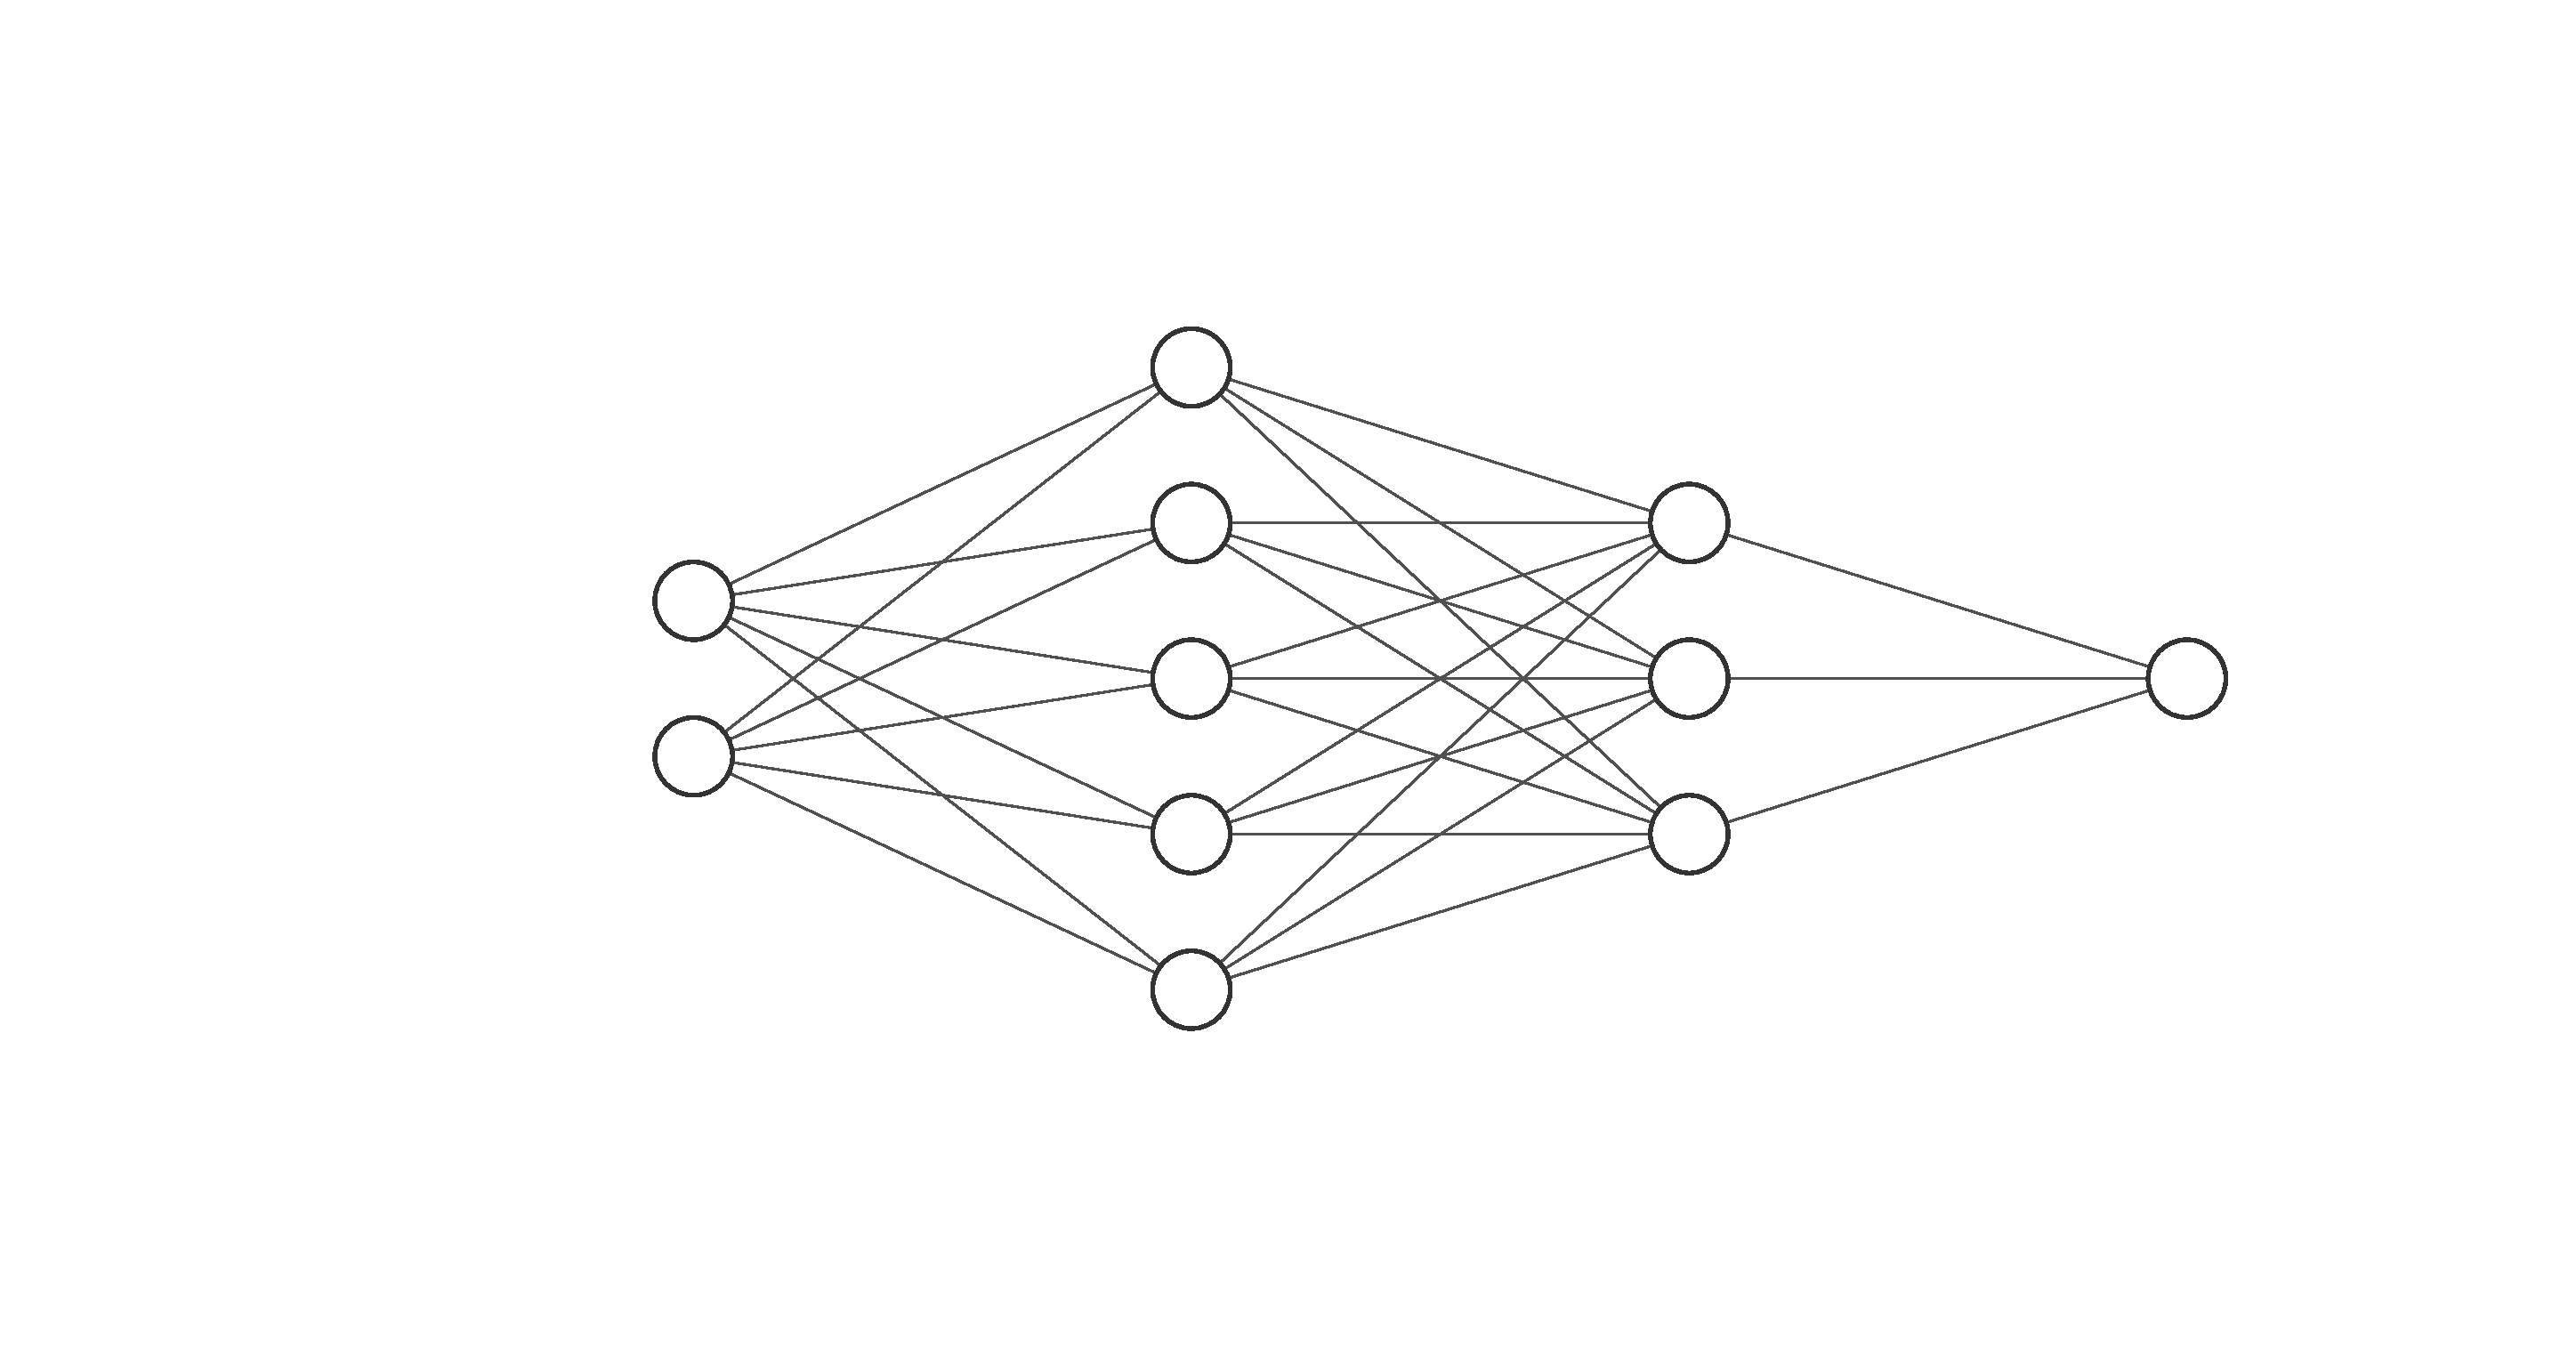
\includegraphics[scale=0.25]{nn31.pdf}
	\end{center}
    \caption{Graphical representation of the neural network used in the NNPDF code.
    For each PDF of Eq.~\eqref{eq:nnpdf31IC_basis} one independent neural network is implemented.}
	\label{nn}                 
\end{figure}
The preprocessing exponents $\alpha_i$ and $\beta_i$ are randomized, by choosing a different value for each replica
within a suitable range. This is determined in a fully self-consistent way: the effective exponents, defined in
Ref.~\cite{Ball:2014uwa} as 
\begin{align}
    \label{eq:effective_exp}
    \alpha_{eff,i}\left(x\right) = \frac{\log q_i\left(x\right)}{\log 1/x}\,, \,\,\,\,
    \beta_{eff,i}\left(x\right) = \frac{\log q_i\left(x\right)}{\log\left(1-x\right)}\,,
\end{align}
are computed for each distribution $q_j$. The $68\%$ confidence level across replicas
is determined for each flavour, and the fit is repeated with the exponents randomized in a range taken equal to twice this 
interval. This procedure is iterated until the range stops changing.

\subsection{Minimization and stopping}
\label{sec:minimization}
The optimal fit is obtained by varying the parameters of $q_j\left(x,Q_0^2\right)$  in such a way that 
some chosen figure of merit is minimized. 
Since most of the experimental data are assumed to have a multigaussian
distribution, a standard choice for such an object is obtained by taking the standard $\chi^2_k $ for each individual 
dataset $k$
\begin{align}
    \label{eq:chi2}
    \chi^2_k 
    =\sum_{ij}^{N_{dat}}\left(D_{ki}-T_{ki}\right)C_{ij}^{-1}\left(D_{kj}-T_{kj}\right)\,,
\end{align}
and then by building the quantity
\begin{equation}
\label{tot chi2}
\chi^2=\sum_k \chi^2_k\,.
\end{equation}
Here $D_{ki}$ is the i-th experimental datapoint in the k-th dataset; $T_{ki}$ is the corresponding 
theoretical prediction, computed using a suitable factorization theorem and 
expressed as a function of the free parameters; 
$C_{ij}$ is the covariance matrix, which takes into account both statistical and systematic uncertainties,
as given by the experimental collaborations.
In order to avoid a fitting bias, multiplicative uncertainties required to be handled with a specific method
denoted as $t_0$ prescription, which as been developed in Ref.~\cite{Ball:2009qv} and implemented in all the following
NNPDF PDFs determination.

%
The $\chi^2$ minimization implemented within the NNPDF environment is based on genetic algorithm (GA):
after a first random initialization of the neural network parameters,
the weights are mutated according to a suitable rule, producing
several copies of the original neural net, each one characterized by a different mutation.
Mutations with the lowest value of the figure of merit are selected and the procedure is iterated.
Different variations of GA have been used in every NNPDF PDFs set, including NNPDF3.1.
Another possible option which has been investigated is the CMA algorithm \cite{DBLP:journals/corr/Hansen16a},
which has been used, for example, in a recent NNPDF determination of 
fragmentation functions \cite{Bertone:2017tyb}. 
Nowadays several efficient deterministic methods are available in a number of public libraries.
As we are going to discuss in the next section, numerical minimizers are no longer the best possible option
and an efficient deterministic minimization is more desirable. 

%
Independently from the specific minimization algorithm implemented, overfitting is avoided
employing a cross-validation technique. In this method, the available data are split
in two sets. The first, the training set, is used for the minimization of the error function,
while the second, the validation set, does not enter the fitting procedure. At each iteration of
the minimization algorithm, the error function between the theory predictions from the neural
net and the data is computed for both the training and validation set. At an early stage of
the training, both these quantities are expected to decrease. However, towards the end of the
training, while the error function over the training set will keep decreasing, the same value
computed over the validation data will reach a minimal value, and eventually it may even start
increasing. This is a signal of overfitting, and the point in parameters space yielding the minimal
value of the validation error is the one taken as the fit result.  

\subsection{Fast Kernel tables}
\label{sec:FK_nnpdf}
In order to get expressions for physical observables, PDFs have to be
evolved up to the physical scale $Q$ of the hard processes and finally 
combined with partonic matrix elements. These steps happen through two separate convolutions, first with
the evolution kernel, see Sec.~\ref{sec:DGLAP}, which solves DGLAP evolution equations and second with the hard cross sections.
Such convolutions happen by means of FastKernel (FK) tables, introduced and validated in Refs.~\cite{Ball:2010de,Bertone:2016lga}
and used in any subsequent NNPDF analysis.
Each PDFs is projected on a suitable basis functions
\begin{align}
    \label{eq:pdf_interpolation_basis}
    q_i\left(x,Q_0^2\right) = \sum_{\alpha}q_i\left(x_{\alpha},Q_0^2\right)\mathcal{I}^{(\alpha)}\left(x\right) 
\end{align}
so that, considering the case of a DIS observable $\mathcal{O}^{\text{DIS}}$, its final value 
can be expressed as a tensors product of the kind  
\begin{align}
    \label{eq:DIS_obs}
    \mathcal{O}^{\text{DIS}} = \left[\text{FK}\right]_{i\alpha}q_{i\alpha}\,.
\end{align}
with the PDF tensor defined as $q_{i\alpha} = q_i\left(x_{\alpha},Q_0^2\right)$.
The matrix $\text{FK}$, denoted as FK table, stores the evolution and partonic matrix element 
and can be precomputed for each process entering the analysis.
In the case of hadronic observables $\mathcal{O}^{\text{DY}}$ 
the PDF tensor has to be replaced by a luminosity tensor $\mathcal{L}_{i\alpha j\beta} = q_{i\alpha}q_{j\beta}$ 
and the FK table becomes a rank-4 tensor,
\begin{align}
    \label{eq:DY_obs}
    \mathcal{O}^{\text{DY}} = \left[\text{FK}\right]_{i\alpha j\beta}\mathcal{L}_{i\alpha j\beta}\,.
\end{align}

%
After computing the value for all the observables entering the fit, the data are split into training and 
validation sets and the $\chi^2$ function of the training set is minimized.



\section{The n3fit environment}
\label{sec:n3fit}
The methodology described in the previous section has been completely revised and extended within the new
{\tt n3fit} environment, first presented in Ref.~\cite{Carrazza:2019mzf}.
In this section we describe the {\tt n3fit} general features, focusing in particular
on the implementation of PDFs positivity and integrability. 
Additionally, we will present some results regarding the problem of the fit basis independence, addressed here for the first time
within this environment.

\subsection{Architecture and general structure}
The {\tt n3fit} code is a python-based framework, written using an object-oriented approach and
a number of external libraries. 
Unlike the previous {\tt c++} code of the NNPDF methodology, 
which is fully based on an in-house implementation of neural networks and minimization algorithms,
in the new framework Keras~\cite{chollet2015keras} and Tensorflow~\cite{tensorflow2015-whitepaper} have been used to deal with them.
This choice greatly simplifies the study of new architectures and techniques recently introduced
in the machine learning literature, allowing for a systematic investigation of many of them, 
and represents an important technological improvement with respect 
to the previous code. 

%
The two main methodological changes in {\tt n3fit} concern the architecture and the minimization algorithm:
rather than using eight independent neural networks, each one giving as output a particular flavour, in
the new environment a single net with an eight-dimensional output is used; additionally, gradient descent
methods are implemented to replace the genetic algorithm described before.
The new architecture, graphically depicted in Fig.~\ref{fig:nn_n3fit}, allows to study and take into account 
cross-correlations between different PDFs,
while the new gradient descent minimizers have been proved to produce more stable fits than those 
obtained using the genetic algorithm. 

\begin{figure}[htb]     
	\begin{center}
		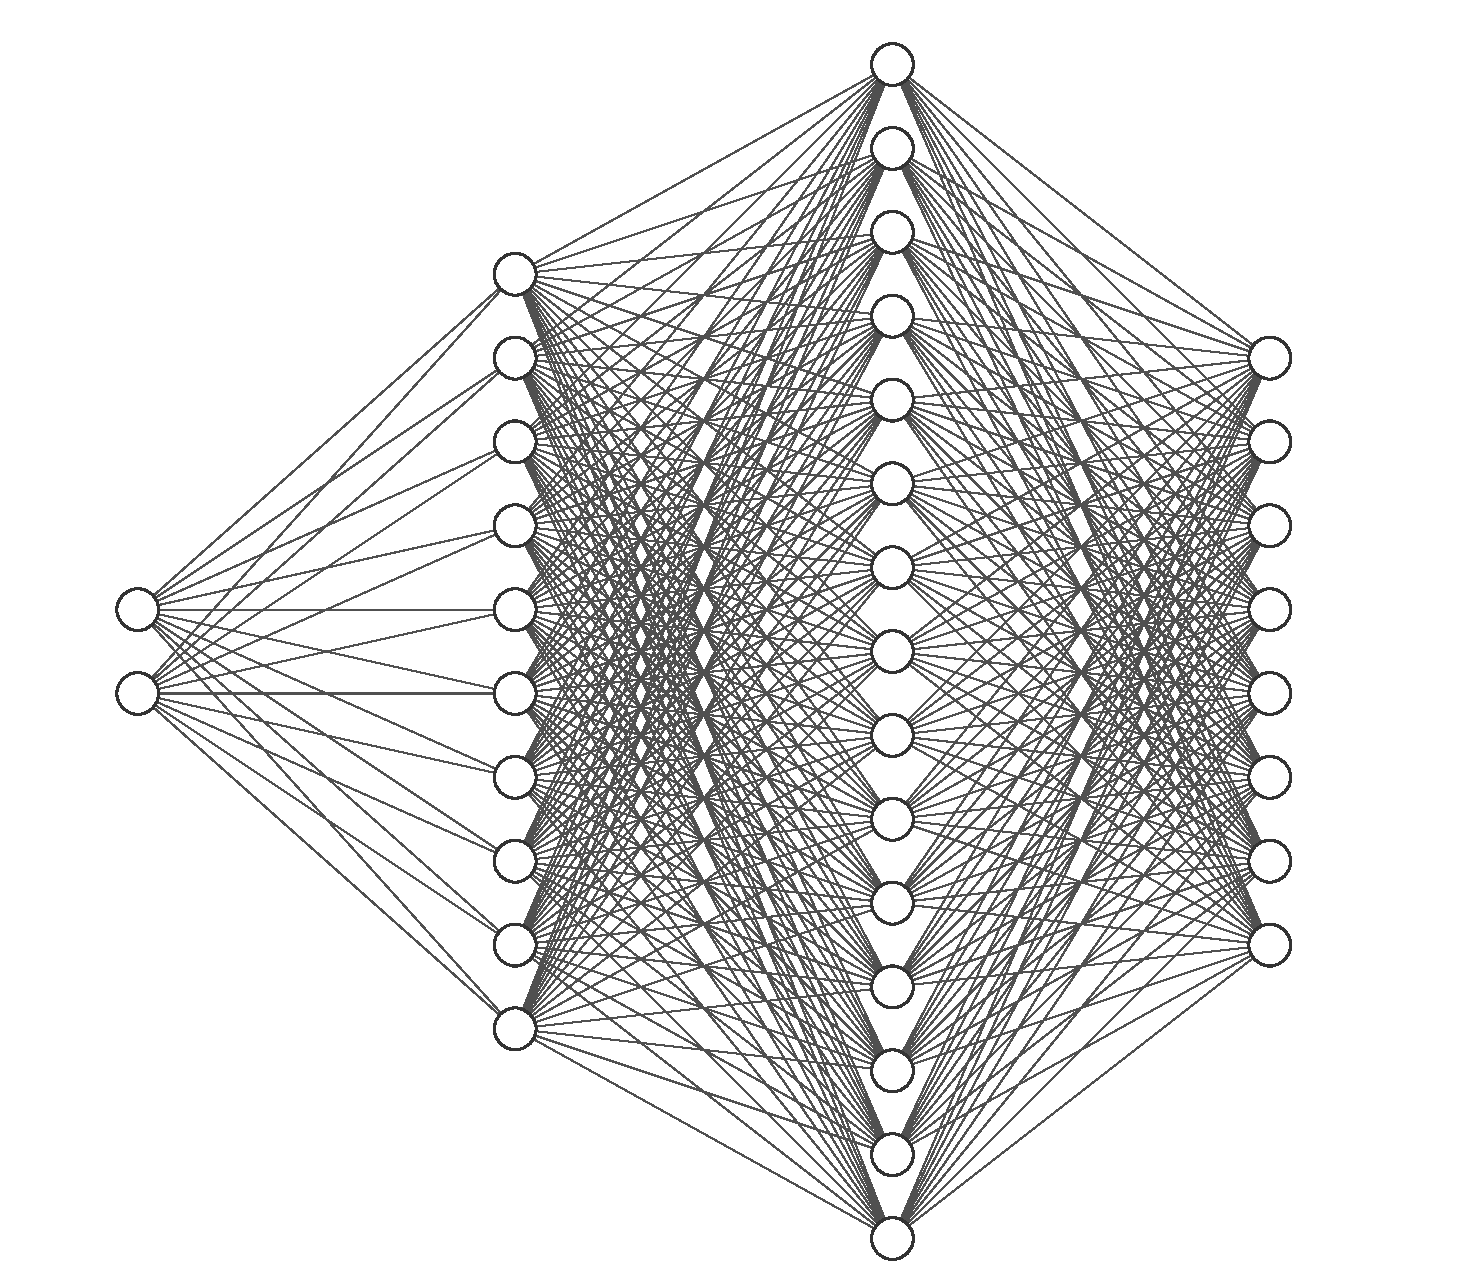
\includegraphics[width=70mm]{nn_n3fit.pdf}
	\end{center}
    \caption{Graphical representation of the neural network used in the {\tt n3fit} framework.
    Each output nodes represents one of the independently parameterized flavours.}
	\label{fig:nn_n3fit}                 
\end{figure}

%
For each dataset entering the fit, a vector of $x$ values is given as input to the neural network and,
as in the old methodology, before going through the intermediate layers it is split into $\left(x,\log x\right)$.
The eight output nodes of the neural network provide the eight independent PDFs parameterized at 
the reference scale $Q_0$. We denote such set of independent parton distributions as \textit{fit basis}.
In NNPDF3.1, this is given by Eq.~\eqref{eq:nnpdf31IC_basis}. The new framework allows the user to choose between 
different options: two standard choices are the so called evolution and flavour basis.
While the former represents the equivalent of the one given in Eq.~\eqref{eq:nnpdf31IC_basis}, in
the latter each quark, antiquark and the gluon are independently parameterized. 
The choice of the fit basis should not affect the final results, however different choices might be more
convenient from a numerical point of view, and different architecture setups might be required
when changing the basis. We will extensively discuss these points in Sec.~\ref{sec:fitbasis}.
Depending on our choice for the fit basis, each output can be supplemented with a suitable preprocessing
polynomials, and with normalization factors to impose momentum and valence sum rules,
as discussed in Sec.~\ref{sec:theory_constraints}

\subsection{Fit basis}
\label{sec:fitbasis}
The parton distributions used to build the FK tables are the thirteen PDFs
\begin{align}
	\label{eq::fkdistributions}
	q_i = \Sigma, g, V, V_3, V_8, V_{15}, V_{24}, V_{35}, T_3, T_8, T_{15}, T_{24}, T_{35}.
\end{align}
Eight of these are independently parameterized, while the remaining ones, involving heavy quarks,
are determined by perturbative evolution, using the matching relations given in Eqs.~\eqref{eq:matching_PDFs}.
When QED corrections are considered in the analysis,
the photon PDF $\gamma$ is also included and independently parameterized.   
As mentioned before, the {\tt n3fit} environment allows for different fit basis choices. In other 
words, the user can choose which distributions should be independently parameterized. 

%
The two most natural choices are the so called \textit{evolution} and \textit{flavour} basis.
The former is defined by the eight dimensional subset of \eqref{eq::fkdistributions} given by 
\begin{align}
    \label{eq:evolution_basis}
    q_k = \left[g, \Sigma, V, V_3, V_8, T_3, T_8, T_{15} \right]\,.
\end{align}
This basis is the equivalent of the one given in Eq.~\eqref{eq:nnpdf31IC_basis}, with the only difference
that the distribution $c^+$ has been replaced by $T_{15}$, defined as 
\begin{align}
    T_{15}     &=  \lp u+\bar{u} +  d+\bar{d} +  s+\bar{s} \rp - 3\lp   c+\bar{c}\rp \, .
\end{align}
In the case of the flavour basis the neural network outputs   
up, down, strange and charm quarks and antiquarks distributions (for charm we consider $c=\bar{c}$) plus the gluon
\begin{align}
    \label{eq:flavour_basis}
	\tilde{q}_k = \left[g, u, \bar{u}, d, \bar{d}, s, \bar{s}, c\right]\,.
\end{align} 
When running a fit, the eight PDFs of the chosen basis are first supplemented with the perturbative heavy quarks
distributions and then rotated back into the FK table basis of Eq.~\eqref{eq::fkdistributions}.

%
The final result of a PDFs determination should be independent on the specific basis used in the fit
and only determined by experimental data and general physical constraints.
The way in which the latter are implemented in the fit can vary depending on the basis,
and might define different final methodologies, which in turn could be more or less convenient
in terms of numerical performances. It is therefore interesting to study different possible
fit basis choices, discussing the differences in performances and methodologies and verifying that,
at least in the kinematic regions where experimental data are available, the 
fit results are independent on the specific PDFs initially parameterized.


\subsection{Theoretical constraints}
\label{sec:theory_constraints}

As mentioned above, there are several theoretical conditions that can be used to further constrain PDFs.
In the following we address each of them, discussing the way they are implemented when considering
different fit bases.

%
\paragraph{Sum rules.}
Energy conservation and the valence structure of the proton imply momentum and valence sum rules
given by 
\begin{align}
    \label{eq:momentum_sumrule}
    \int_0^1 dx\, x\left(g\left(x\right) + \Sigma\left(x\right)\right) = 1\,. 
\end{align}
and
\begin{align}
    \label{eq:valence_sumrules}
    \int_0^1& dx\, V\left(x\right) = \int_0^1 dx\, V_8\left(x\right) = 3\,,   \,\,\,
    \int_0^1 dx\, V_3\left(x\right) = 1\,.
\end{align} 
These are implemented in the fit multiplying the distributions $V$, $V_3$, $V_8$ and $g$ by suitable normalization factors
$A_V$, $A_{V_3}$, $A_{V_8}$ and $A_g$ defined as
\begin{align}
    A_V = A_{V_8} = \frac{3}{\int_0^1 dx\, V\left(x\right)}\,,\,\,
    A_{V_3} = \frac{1}{\int_0^1 dx\, V_3\left(x\right)}\,,\,\,
    A_g = \frac{1 - \int_0^1 dx\, x \Sigma\left(x\right)}{\int_0^1 dx\, x g\left(x\right)}\,,
\end{align} 
so that Eqs.~\eqref{eq:momentum_sumrule}, \eqref{eq:valence_sumrules} are automatically
satisfied.
Such multiplication happens after rotating the fit basis back into Eq.~\eqref{eq::fkdistributions},
so that the procedure remains the same independently on the choice of the fit basis.


\paragraph{Large- and small-$x$ behaviour.} 
The large-$x$ behaviour of the PDFs has to be consistent with the elastic limit, namely the condition
$q_i\left(x=1\right)=0$ has to be satisfied by all the distributions of both the flavour and evolution basis.
This can be easily implemented in the fit by supplementing the neural network parameterization of 
each flavour by the preprocessing factor $\left(1-x\right)^{\beta_i}$, just like in the NNPDF methodology
described before.
The use of an additional polynomial factor $x^{-\alpha_i}$, controlling the small-$x$ behaviour of each flavour,
only makes sense when working in the evolution basis. In this case, each flavour is either a singlet or nonsinglet
distribution, and as such its small-$x$ behaviour can be classified as integrable (nonsinglet) or not integrable (singlet)
in $x=0$: a parameterization like the one given in Eq.~\eqref{eq::paramEvol} can be used, with $\alpha$
randomized in intervals such that $\alpha<1$ in the former case and $\alpha>1$ in the latter.
%
On the other hand, when working in the flavour basis each distribution (except the gluon) has both a singlet 
and a nonsinglet component, which makes it impossible to use a polynomial expression 
to describe in a consistent way its small-$x$ behaviour. Because of this, when working in the flavour basis
only a large-$x$ preprocessing is implemented, so that each distribution of Eq.~\eqref{eq:flavour_basis} is
parameterized as
\begin{align}
    x\,\tilde{q}_j\left(x, Q_0^2\right) = \left(1-x\right)^{\beta_{j}}\text{NN}_{j}\left(x\right)\,,
\end{align}
with $\text{NN}_{j}\left(x\right)$ denoting the corresponding neural network output, just as in Eq.~\eqref{eq::paramEvol}.



\paragraph{Positivity.}
As recalled in chapter~\ref{ch:fact}, PDFs are renormalization scheme dependent quantities.
Despite at LO they can be interpreted as probabilities distributions, when considering QCD corrections
such naive picture doesn't hold any more. This in general prevents PDFs from being positive definite objects.
However, regardless of the PDFs sign and shape, cross sections for high-energy processes have to be positive,
which means that fit solutions leading to negative cross-sections have to be discarded.
This condition might have a non-negligible impact on the PDFs themselves, 
especially in those kinematic regions where no experimental
data are available: functional forms giving negative cross sections cannot be 
physical solutions of the problem, and therefore should be discarded.  
In the old {\tt c++} code such requirement is implemented through the use of Lagrange multipliers, 
penalizing fit solutions for which a set of chosen high-energy cross sections,
denoted as positivity observables, result to be negative.

%
It would be highly beneficial to work in a renormalization scheme in which PDFs are positive definite
also beyond LO: this would allow to implement directly the positivity of the distributions,
without having to rely on a specific choice of positivity observables.
This is indeed the idea of a recent paper~\cite{Candido:2020yat}, where such positive renormalization
scheme for PDFs is built. In the same paper, the Authors work out the relation between such positive
renormalization scheme and the standard $\overline{MS}$ scheme, which is the one commonly used in 
PDFs determinations, and surprisingly they find out that NLO $\overline{MS}$ distributions
for quarks, antiquarks and gluon are actually positive definite.  
This result has been accounted for in {\tt n3fit}, where positivity is imposed at the PDFs level.
In the following we describe how this feature is implemented in the code, and we assess the impact of such constraint
on the large-$x$ region of the PDFs.

%
For each distribution $\tilde{q}_k$ which has to be positive, namely for all the PDFs defining the
flavour basis of Eq.~\eqref{eq:flavour_basis}, we add to the total $\chi^2$ a contribution defined as  
\begin{align}
	\label{eq:chi2pos_k}
	\chi^2_{k,pos} = \Lambda_k \,\sum_i \,\text{Elu}_{\alpha}\left(-\tilde{q}_k\left(x_i,Q^2\right)\right)\,,
\end{align}
with $Q^2 = 5\, \text{GeV}^2$, $x_i$ given by 10 points logarithmically spaced between $5\cdot10^{-7}$ and $10^{-1}$ and 10 points
linearly spaced between $0.1$ and $0.9$. The Elu function is defined as 
\begin{align}
	\label{eq:Elu}
	\text{Elu}_{\alpha}\left(t\right) = 
	\begin{cases}
		t \,\,\,\,\,\,\,\,\,\,\,\,\,\,\,\,\,\,\,\,\,\,\,\,\,\,\,\,\,\,\text{if}\,\,\,\, t>0 \\
		\alpha\left(e^t-1\right)\,\,\,\,\,\,\,\text{if}\,\,\,\, t<0
	\end{cases}\,,
\end{align} 
with $\alpha=10^{-7}$. 
When the distribution $\tilde{q}_k\left(x_i, Q^2\right)$ is negative, the total $\chi^2$ will receive a positive contribution
(a penalty) proportional to the corresponding Lagrange multipliers $\Lambda_k$. 
Therefore, during the minimization of $\chi^2_{tot}$ solutions corresponding to positive distributions $q_k$
will be favoured. Note that such implementation works fine for both the evolution and flavour basis, the only 
difference being the linear transformation mapping the network outputs to the positive distributions to be 
used in Eq.~\eqref{eq:chi2pos_k}.

\paragraph{Integrability.}
Given the lack of data in the small-$x$ region, when $x<10^{-4}$ the PDFs are left largely unconstrained. 
Because of the redundant parameterization employed in the NNPDF methodology, this will result in 
an artificially big PDFs error in the small-$x$ region.
This is an important feature that a reliable PDFs set should have: in those kinematic regions where experimental data
are missing, the PDFs error should increase accordingly.
There are however some physical considerations that can be made to further constrain PDFs at small-$x$, 
which can be used to reduce the huge error band in this kinematic region. 
In order to have well defined momentum and valence sum rules the distributions $V, V_3, V_8, xg, x\Sigma$ 
have to be integrable when $x$ decrease to zero.
Moreover, in order to have well defined Gottfried sum rules, also the integrals of $T_3$ and $T_8$ over the interval
$\left(0,1\right)$ have to be finite. 

This means that, denoting as $q\left(x,Q_0^2\right)$ a generic integrable PDF at the fitting scale, as $x$ decreases to zero
such distribution cannot raise faster than $1/x$. In other words the following limit has to be verified
\begin{align}
    \label{eq:integrability}
    \lim_{x\rightarrow 0} xq\left(x,Q_0^2\right) = 0\,.
\end{align}
%
In order to satisfy numerically Eq.~\eqref{eq:integrability}
we require that, for a given set of points $x^{(i)}_{\text{integ}}$ in the small-$x$ region,
the function $xq\left(x\right)$ evaluated in these points is much smaller than its peak value,
\begin{align}
    \label{eq:integ_def}
    \sum_i|xq|_{x=x^{(i)}_{\text{integ}}} \ll xq|_{x=x_{\text{peak}}}\,,
\end{align}
with $x_{\text{peak}}$ denoting the point where the distribution $xq$ reaches its maximum value.
Eq.~\eqref{eq:integ_def} can be rewritten introducing a numerical parameter $f_q$ of order $10^{-1}$
\begin{align}
    \label{eq:integ_def_2}
    \sum_i|xq|_{x=x^{(i)}_{\text{integ}}} < f_q*xq|_{x=x_{\text{peak}}}\,.
\end{align}
Despite Eq.~\eqref{eq:integ_def_2} is not mathematically equivalent to Eq.~\eqref{eq:integrability},
 the idea is that,
if satisfied for small enough $x$ values $x^{(i)}_{\text{integ}}$, the function $xq\left(x\right)$ will 
decrease to zero as $x$ keeps getting smaller, and the integrals defining the sum rules will be 
well defined. Also, unlike Eq.~\eqref{eq:integrability}, the condition given
in Eq.~\eqref{eq:integ_def_2} can be easily verified replica by replica, so that replicas not satisfying it
can be discarded.

%
In a similar way to what done for positivity we can impose integrability. 
For each distributions $q_k$ which has to be integrable we
add to the total $\chi^2$ a new bit defined as  
\begin{align}
	\label{eq:chi2integ_k}
	\chi^2_{k,integ} = \Lambda_k \,\sum_i \,\left[x_i\,q_k\left(x_i,Q^2\right)\right]^2\,,
\end{align}
In this way, the fit will favour configurations with smaller values of $|x_i\,q_k\left(x_i,Q^2\right)|$, and should 
therefore produce distributions satisfying Eq.~\eqref{eq:integ_def_2}. The points $x_i$ are chosen in different ways depending
on the specific distribution and fit basis we are considering, as detailed in the next section. 


\subsection{Results}
\label{sec:results_nnpdf}
In the previous section we have described how theoretical constraints are implemented in the fit.
In particular we have seen how, when imposing positivity and integrability,
the total experimental $\chi^2$ has to be supplemented by additional contributions
proportional to Lagrange multipliers, so that the total $\chi^2$ which is actually minimized
during the fit is 
\begin{align}
	\label{eq:chi2pos_integ}
	\chi^2_{tot} = \chi^2_{exp} + \sum_k\, \chi^2_{k,\text{pos}} + \sum_l\, \chi^2_{l,\text{integ}}
\end{align}
with the indices $k$ and $l$ running on the positive and integrable distributions
and $\chi^2_{k,\text{pos}}$, $\chi^2_{l,\text{integ}}$ defined in Eqs.~\eqref{eq:chi2pos_k}, \eqref{eq:chi2integ_k}.

%
In this section we present results produced with the new {\tt n3fit} methodology,
focusing on the effects positivity and integrability constraints have on the final result.
Our point here is to show the effects of such theoretical constraints on a given baseline which doesn't 
include them. We will first present results obtained using the evolution basis, and in the
next section we will repeat the exercise in the flavour basis, in order to check explicitly 
fit basis independence.
%Such analysis, together with a detailed comparison with NNPDF3.1 and an extended version
%of the baseline dataset, will be part of the NNPFD4.0 release paper.

%
The baseline dataset we will consider here is the one of the NNPDF3.1 PDFs set, presented and discussed in Ref.~\cite{Ball:2017nwa}.
This includes: fixed-target neutral-current 
(NC) DIS structure function data from NMC~\cite{Arneodo:1996kd,Arneodo:1996qe}, 
SLAC~\cite{Whitlow:1991uw} and BCDMS~\cite{Benvenuti:1989rh}; charged-current 
(CC) DIS structure function data from CHORUS~\cite{Onengut:2005kv} and 
NuTeV~\cite{Goncharov:2001qe,Mason:2006qa}; HERA data from their combined 
measurements~\cite{Abramowicz:2015mha}, including charm-production cross 
sections~\cite{Abramowicz:1900rp} and $b$-tagged structure 
functions~\cite{Aaron:2009af,Abramowicz:2014zub}; fixed-target Drell-Yan data 
from E866~\cite{Webb:2003ps,Webb:2003bj,Towell:2001nh} and 
E605~\cite{Moreno:1990sf}; collider Drell-Yan data from 
CDF~\cite{Aaltonen:2010zza} and D0~\cite{Abazov:2007jy,
Abazov:2013rja,D0:2014kma}; and Drell-Yan, inclusive gauge boson, and top-pair
production data from 
ATLAS~\cite{Aad:2013iua,Aad:2014qja,Aad:2011dm,Aaboud:2016btc,Aad:2015auj,
Aad:2014kva,Aaboud:2016pbd,Aad:2015mbv}, CMS~\cite{Chatrchyan:2012xt,
Chatrchyan:2013mza,Chatrchyan:2013tia,Khachatryan:2016pev,Khachatryan:2015oaa,
Khachatryan:2016mqs,Khachatryan:2015uqb,Khachatryan:2015oqa} 
and LHCb~\cite{Aaij:2012vn,Aaij:2012mda,Aaij:2015gna,Aaij:2015zlq}. 
In total this baseline dataset contains $n_{\rm dat}=4287$
datapoints, see Ref.~\cite{Ball:2017nwa} for more details.

\comment{You took this list from the jets paper, but there you have 3813 datapoints.
The difference is that in the jet paper the baseline doe not include jets data which are included in NNPDF31. You
have checked this looking at the runcards} 

%
When working in the evolution basis the small-$x$ behaviour is largely controlled by the preprocessing
polynomial factor. Integrability (as defined in Eq.~\eqref{eq:integ_def_2})
can then be satisfied mainly by choosing the corresponding preprocessing exponents in an interval which ensures integrability.
Additionally, the lagrange multiplier term given in Eq.~\eqref{eq:chi2integ_k} is added to the
total $\chi^2$ using a single small-$x$ point $x=10^{-9}$. These choices have been proved to
produce replicas which mostly satisfy Eq.~\eqref{eq:integ_def_2}. 

%
In Tab.~\ref{tab:experiments_chi2} we provide values of $\chi^2/N_{\text{dat}}$ for an {\tt n3fit } global fit,
reporting results also for each experiment included in the analysis.
These are compared to their {\tt n3fit} counterpart produced without positivity and integrability constraints. 
Inspection of this table shows how the fit quality is basically unaffected by the introduction of the
theoretical constraints, with a slight improvement in the total $\chi^2$. Such mild improvement provides an
additional confirmation of the validity of our theoretical constraints: despite these represent additional 
conditions to be satisfied during the fit, they provide meaningful physical hints, making it easier to describe 
the experimental data.
 
%
In Fig.~\ref{fig:distances} we show the distance between the two fits, quantifying the effect of theoretical
constraints at the PDFs level. For the definition of the distance between PDFs sets, see App.~\ref{app:estimators}.
While in the small-$x$ region the difference between the two fits remains below 
one-sigma, in the medium- and large-$x$ regions we find differences of up to
two-sigmas. The evolution basis flavours $V$, $V_3$, $V_8$ and $T_8$ are plotted in linear scale in Fig.~\ref{fig:pdfs_plots}.
Inspection of these plots show an important reduction of the PDFs error for the flavours $V$, $V_3$, $V_8$,
and a change in the PDFs shape and central value to satisfy the new positivity constraints, which affects also the distribution
$T_8$.

%
We conclude that overall after the inclusion of theoretical constraints the fit provides an equivalent,
or slightly better, description of the input data. However there are important differences at the level of the PDFs,
whose replicas are globally shifted in order to satisfy positivity, resulting in a general decreasing in the PDFs error,
and in a non negligible change in their central value.

\begin{table}[htbp!]
    \centering
    %%%%%%%%%%%%%%%%%%%%%%%%%%%%%%%%%%%%%%%%%%%%%%%%%%%%%%%
\begin{center}
    \renewcommand*{\arraystretch}{1.50}
    \small
  \begin{tabularx}{\textwidth}{Xrccc}
  \toprule
  Experiment    & $N_{\rm dat}$ & $\chi^2_{\rm evol}$ & $\chi^2_{\rm flav}$    & Baseline $\chi^2$     \\
  \midrule
  NMC   & 325 & 1.247 & 1.258  & 1.280     \\
  SLAC  & 67  & 0.733 & 0.757  & 0.721    \\
  BCDMS & 581 & 1.183 & 1.130  & 1.253 \\
  CHORUS & 832 & 1.159 & 1.108  & 1.122 \\
  NTVDMN & 76   & 0.969 & 1.332 & 0.961 \\
  HERACOMB & 1145 & 1.150 & 1.125 & 1.168 \\
  HERAF2CHARM & 37 & 1.522 & 1.572 & 1.492 \\
  F2BOTTOM & 29 & 1.100 & 1.100 & 1.112 \\ 
  DYE886 & 104 & 1.410 & 1.534 & 1.560 \\
  DYE605 & 85 & 1.143 & 1.161 & 1.157 \\ 
  CDF & 105 & 0.969 & 0.921 & 0.996 \\
  D0 & 48 & 1.505 & 1.362 & 1.409 \\
  ATLAS & 360 & 1.105 & 1.082 & 1.126 \\
  CMS & 408 & 1.035 & 1.056 & 1.052 \\
  LHCb & 85 & 1.438 & 1.320 & 1.526 \\
  \bottomrule
  Total & 4287 & 1.153 & 1.136 & 1.171 \\
  \bottomrule
  \end{tabularx}
  \end{center}
  %%%%%%%%%%%%%%%%%%%%%%%%%%%%%%%%%%%%%%%%%%%%%%%%%%%%%%%%%%
  
    \caption{The values of $\chi^2/N_{\rm dat}$ for each experiment included in the global fit, before and
    after the inclusion of positivity and integrability constraints. Values are reported for fits in both the evolution and flavour 
    basis.}
    \label{tab:experiments_chi2}
\end{table}

\begin{figure}[t!]
    \begin{center}
        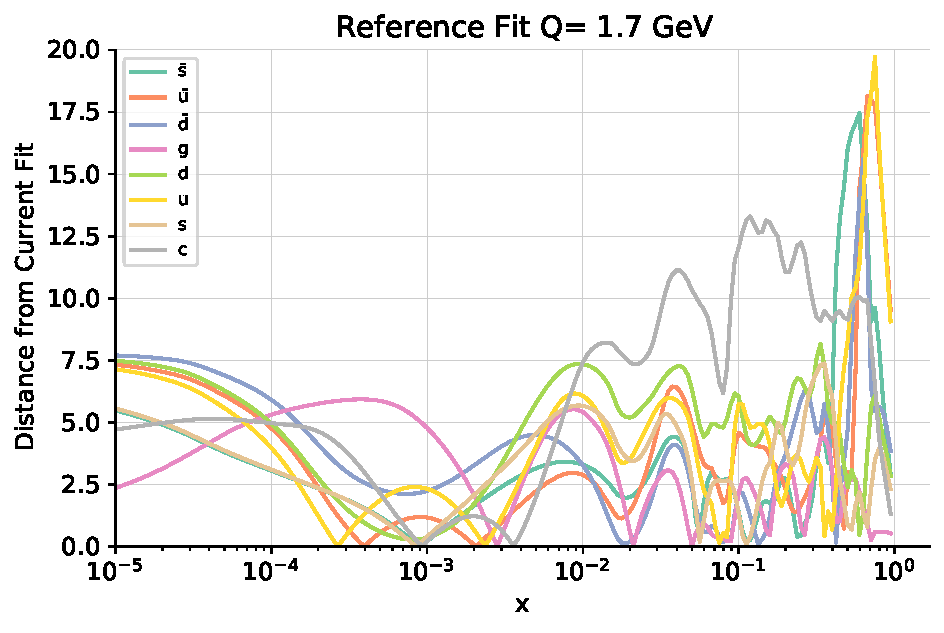
\includegraphics[width=0.49\linewidth]{normalize_basespecs0_pdfscalespecs0_distspecs0_plot_pdfdistances.pdf}
        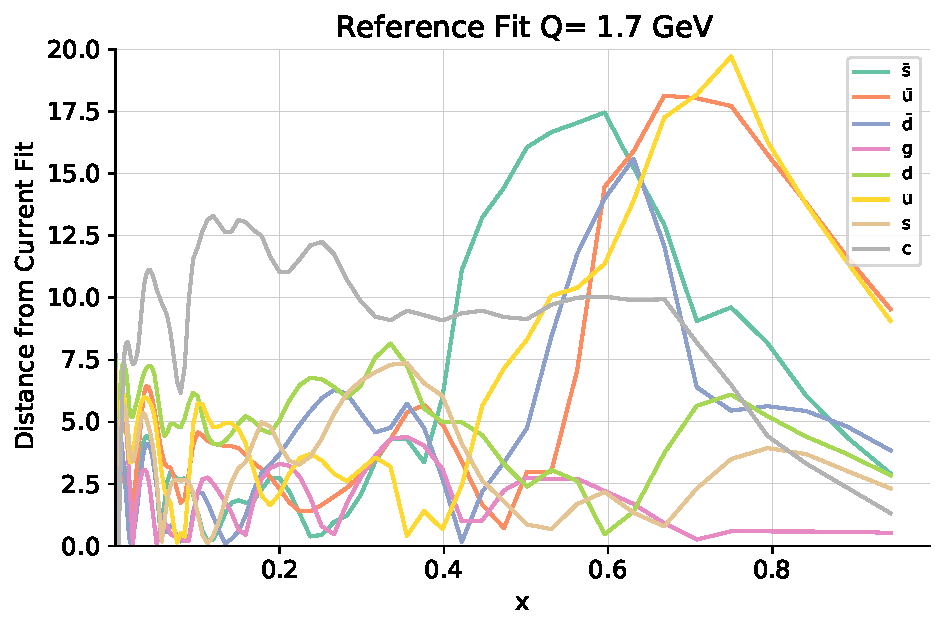
\includegraphics[width=0.49\linewidth]{normalize_basespecs0_pdfscalespecs1_distspecs0_plot_pdfdistances.pdf}
        \caption{Distance plots} 
        \label{fig:distances} 
    \end{center}
\end{figure}

\begin{figure}[t!]
    \begin{center}
        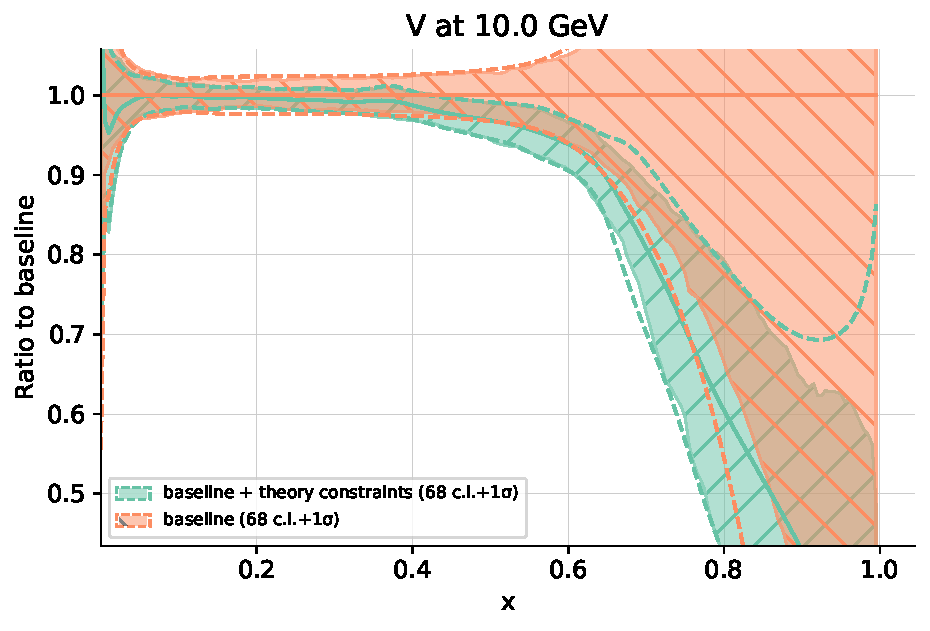
\includegraphics[width=0.49\linewidth]{plot_pdfs_V.pdf}
        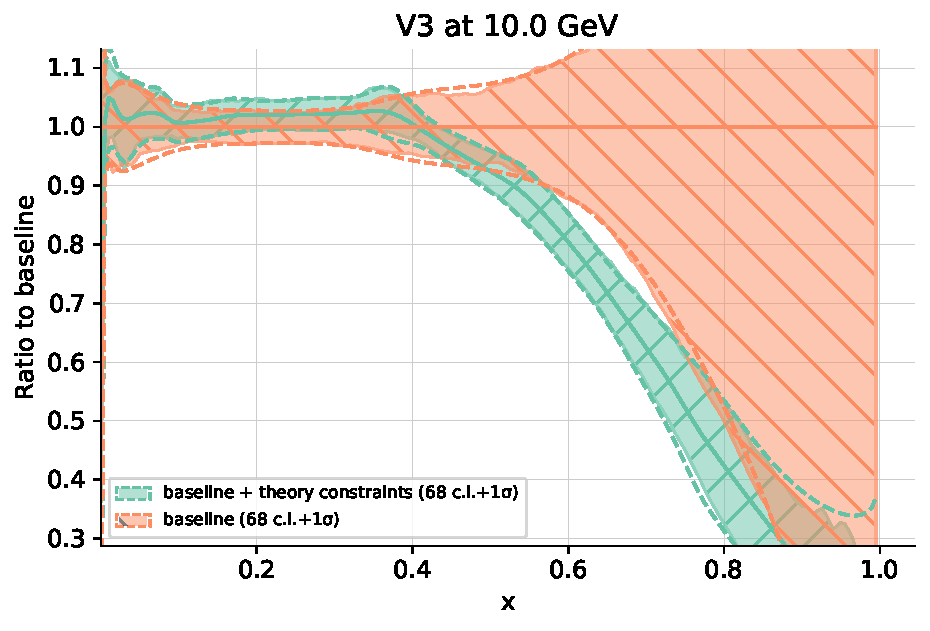
\includegraphics[width=0.49\linewidth]{plot_pdfs_V3.pdf}
        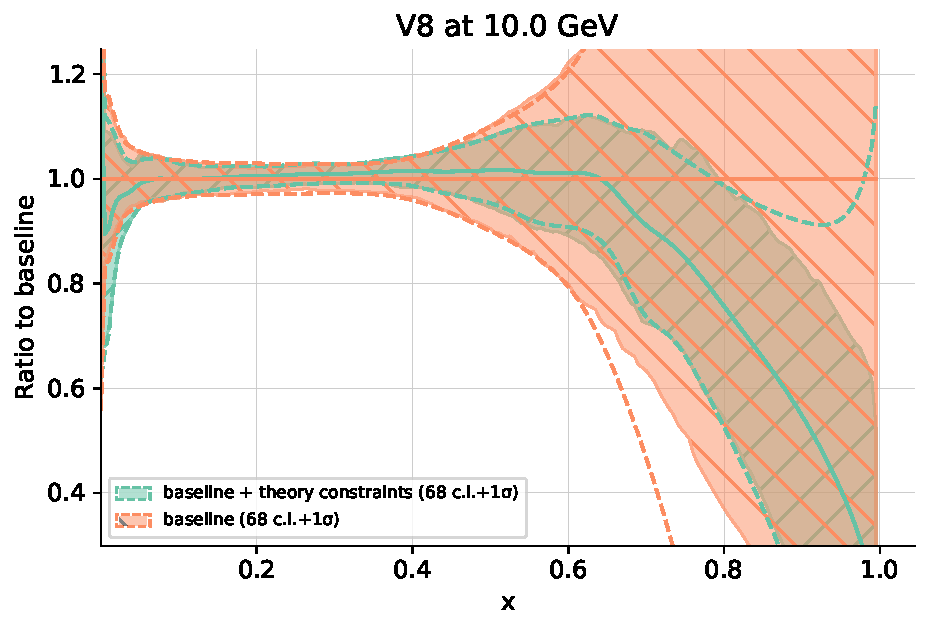
\includegraphics[width=0.49\linewidth]{plot_pdfs_V8.pdf}
        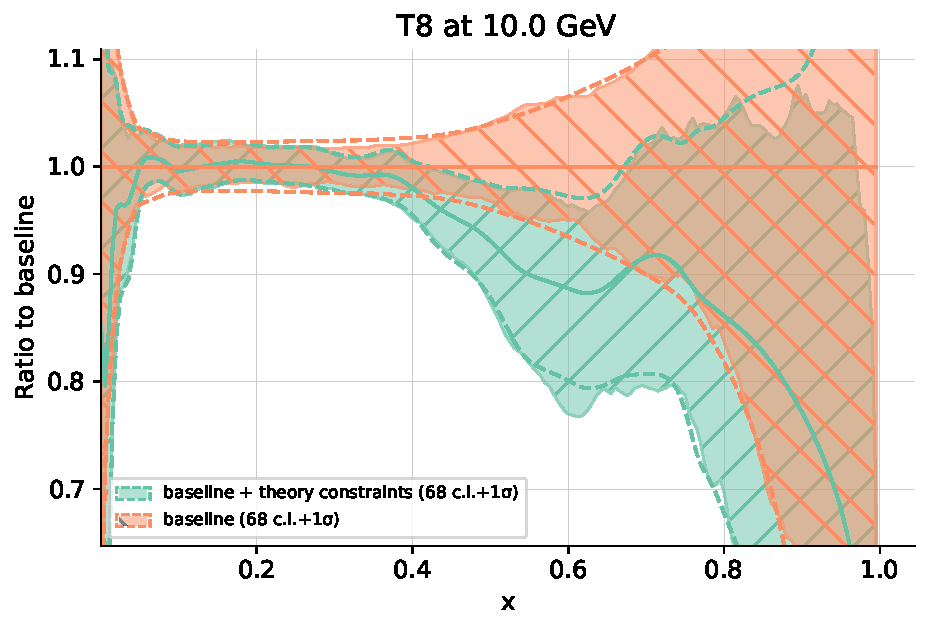
\includegraphics[width=0.49\linewidth]{plot_pdfs_T8.pdf}
        \caption{PDFs plots} 
        \label{fig:pdfs_plots} 
    \end{center}
\end{figure}


\subsection{Fit basis independence}
As described in Sec.~\ref{sec:fitbasis}, different choices for the specific PDFs which are independently
parameterized are possible.
In this section we present results for a fit run in the flavour basis, using the same methodology
implemented for the evolution basis (same minimization algorithm and architecture parameters) 
and imposing the theoretical constraints as described previously.

%
As mentioned in Sec.~\ref{sec:theory_constraints}, when working in the flavour basis 
no small-$x$ preprocessing is used. This implies that the small-$x$ behaviour of the PDFs, which is unconstrained 
by experimental data, can only be controlled through Lagrange multipliers.
Because of this reason, for integrable distributions more stringent constraints are used than those implemented
for the evolution basis. In particular, in order to get replicas satisfying Eq.~\eqref{eq:integ_def_2},
the lagrange multiplier terms given in Eq.~\eqref{eq:chi2integ_k} are built using the three small-$x$
points $x_i = 10^{-5}, 10^{-4}, 10^{-3}$. 

%
The fit quality is again basically unchanged, with a total $\chi^2$ which is slightly better than the corresponding 
value in the evolution basis: $\chi_{\text{flav}}^2=1.13$ to be compared with the value $\chi_{\text{evol}}^2=1.15$ 
from Tab.~\ref{tab:experiments_chi2}.
The resulting PDFs plotted in the evolution basis are reported in Fig.~\ref{fig:pdfs_plots_flav_vs_evol}, 
where they are compared with the evolution basis fit presented in the previous section.
The plots are shown in linear scale, in order to highlight the $x$-region where experimental data lay.
By inspection of Fig.~\ref{fig:pdfs_plots_flav_vs_evol} it is clear that fit basis independence is achieved,
showing how, as expected, as long as data are present and physical constraints given by positivity, integrability and sum rules
consistently implemented, different choices for the fit basis do no change the final results.
It is worth recalling that this result, even if expected, is not trivial. When we change fit basis a number
of settings and parameters are changed at the same time. In particular, no small-$x$ preprocessing
is used for the flavour basis, which as a consequence present a lower number of free parameters.
The fact that we still get equivalent results provides a strong validation check of the {\tt n3fit} environment.

%
In order to determine the best methodology, one should fix the input dataset and the fit basis. Once this is done,
a scan of the hyperparameters defining the final methodology has to be performed 
(neural network architecture, minimization algorithm, positivity and integrability parameters ...), in order to determine
the corresponding values which allow the best fit.
The methodology used to produce the results presented here has been optimized considering the evolution basis,
which will be used in the final NNPDF4.0 release.  
If results in the flavour basis were to be used to do actual phenomenology, an additional hyperparameters scan
should be run, to ensure the best possible performance of the methodology. 
Here we have shown how, without explicitly doing an additional hyperoptimization, the {\tt n3fit} environment still
allows to obtain a good fit using a different basis, providing a proof of concept of basis independence.


\begin{figure}[t!]
    \begin{center}
        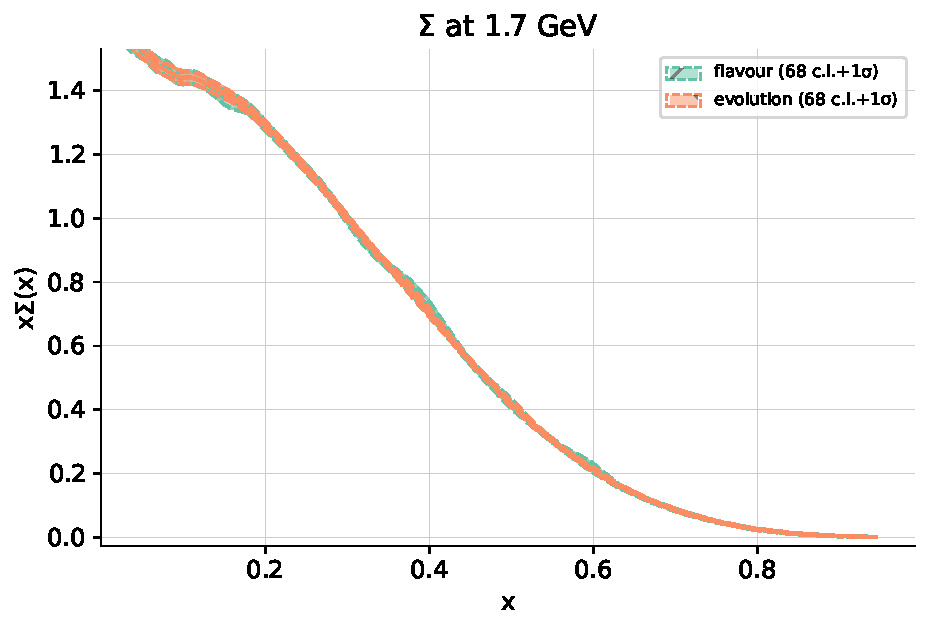
\includegraphics[width=0.49\linewidth]{plot_pdfs_Sigma_flav_vs_evol.pdf}
        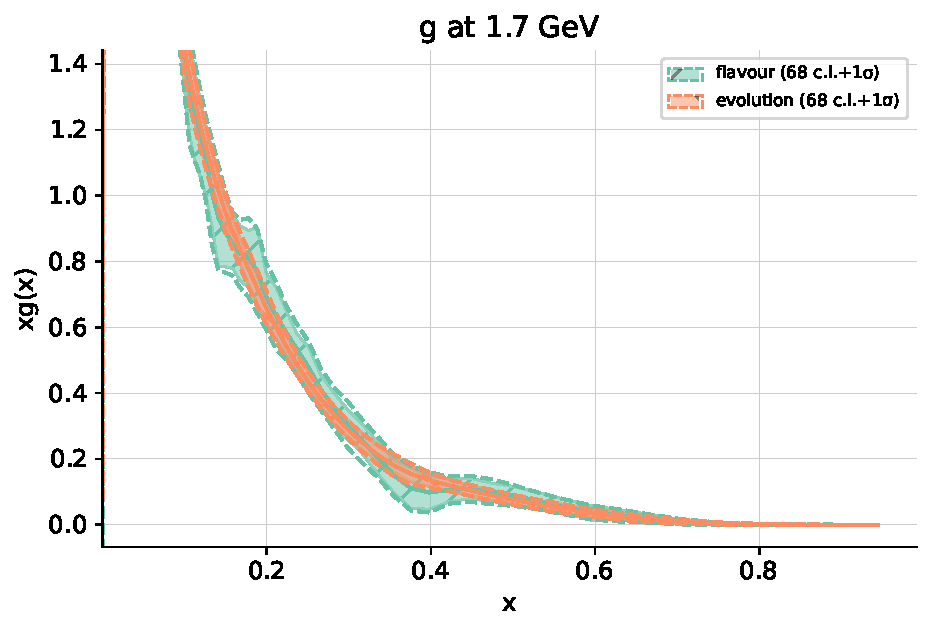
\includegraphics[width=0.49\linewidth]{plot_pdfs_g_flav_vs_evol.pdf}
        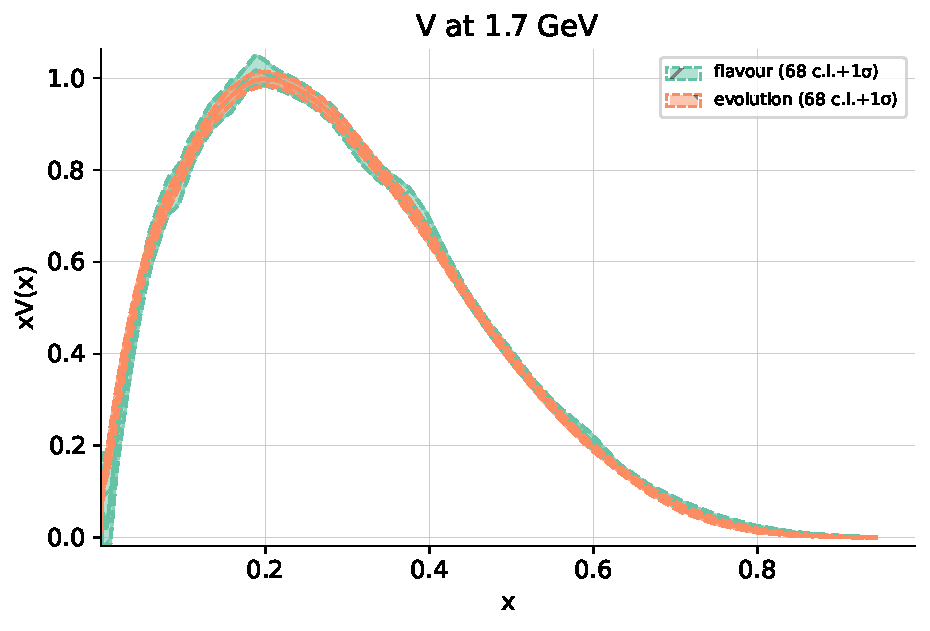
\includegraphics[width=0.49\linewidth]{plot_pdfs_V_flav_vs_evol.pdf}
        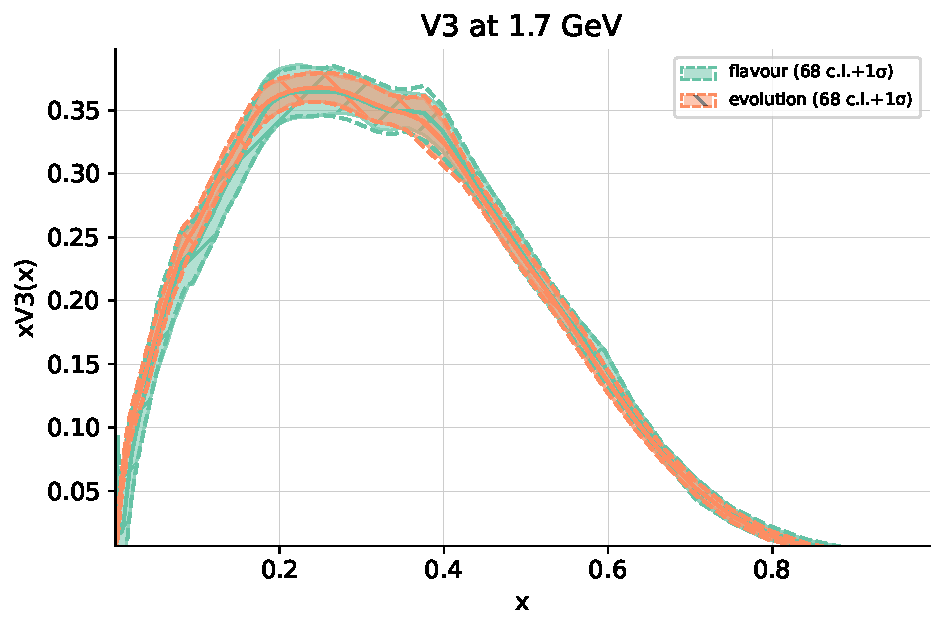
\includegraphics[width=0.49\linewidth]{plot_pdfs_V3_flav_vs_evol.pdf}
        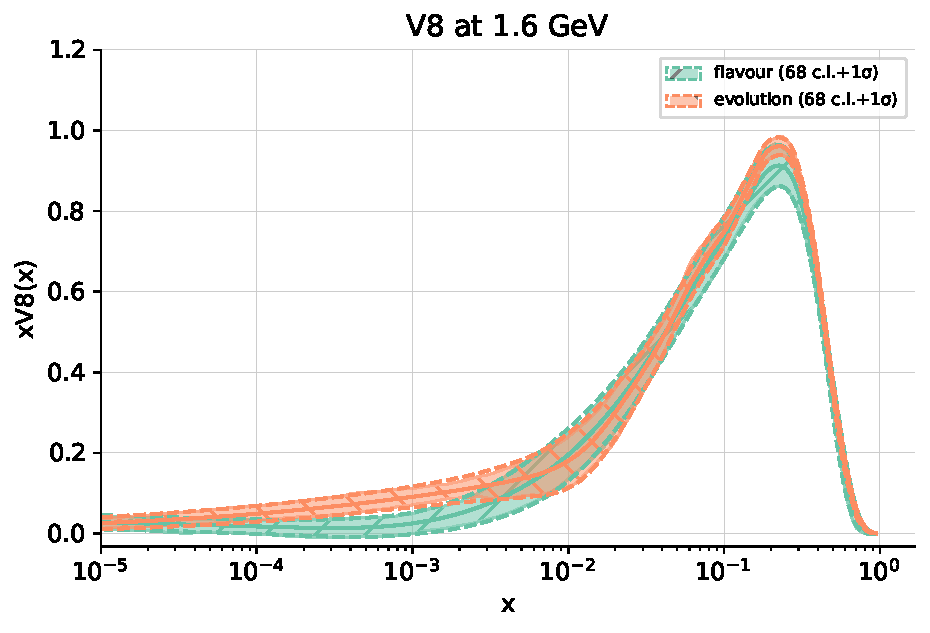
\includegraphics[width=0.49\linewidth]{plot_pdfs_V8_flav_vs_evol.pdf}
        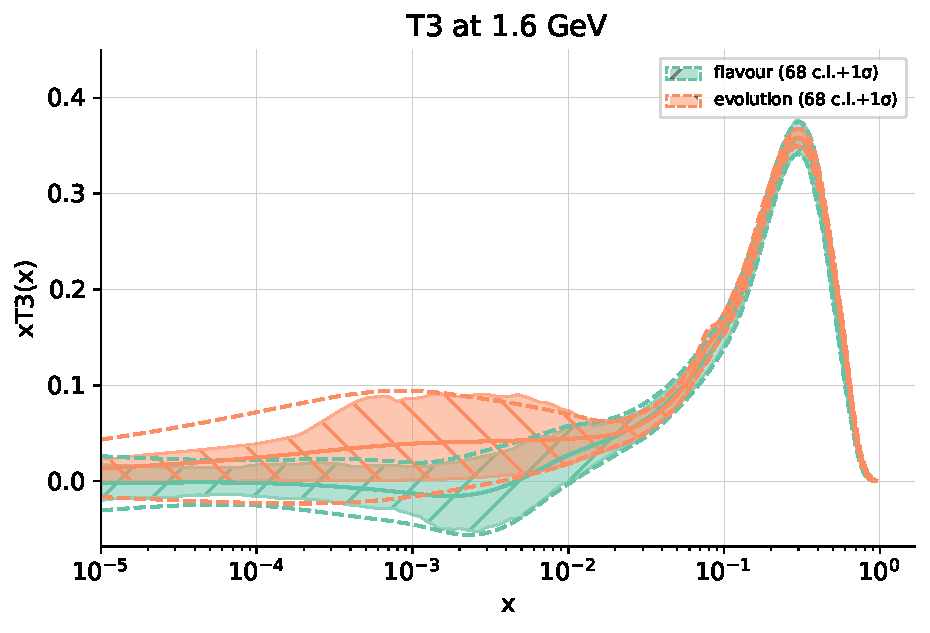
\includegraphics[width=0.49\linewidth]{plot_pdfs_T3_flav_vs_evol.pdf}
        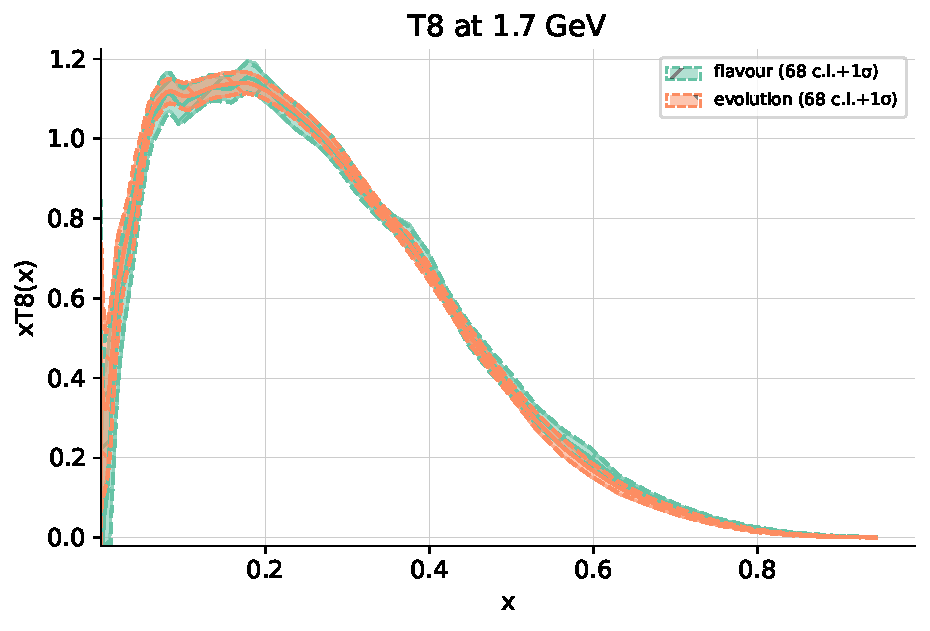
\includegraphics[width=0.49\linewidth]{plot_pdfs_T8_flav_vs_evol.pdf}
        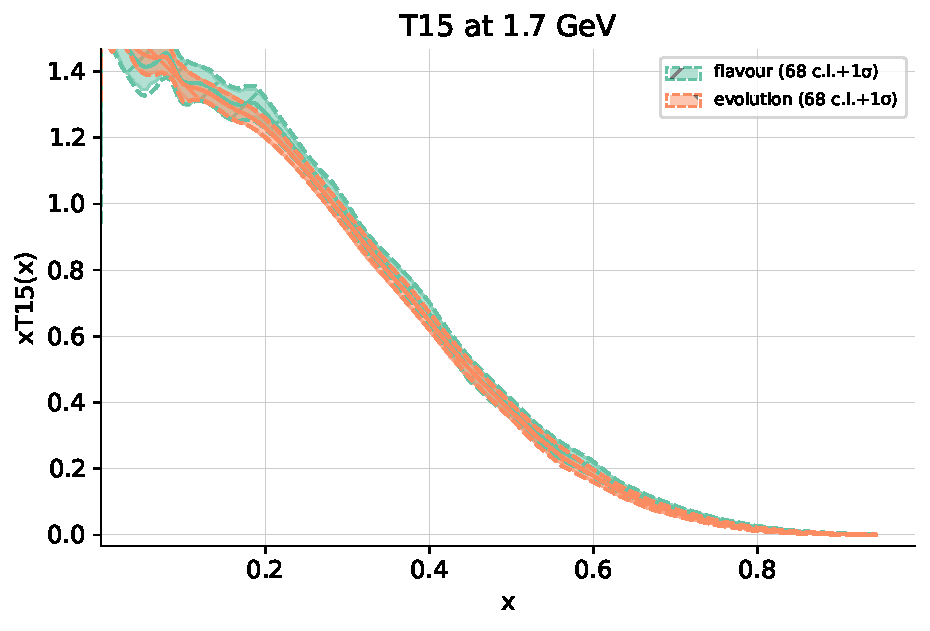
\includegraphics[width=0.49\linewidth]{plot_pdfs_T15_flav_vs_evol.pdf}
        \caption{PDFs plots comparing results for fits performed in the evolution (orange) and flavour (green) basis.} 
        \label{fig:pdfs_plots_flav_vs_evol} 
    \end{center}
  \end{figure}



